\documentclass[11pt,a4paper]{article}
\usepackage[T1]{fontenc}
\usepackage[utf8]{inputenc}
\usepackage{lmodern}
\usepackage[margin=2.2cm]{geometry}
\usepackage{amsmath,amssymb}
\usepackage{booktabs,tabularx,array}
\usepackage{xcolor}
\usepackage{graphicx}
\usepackage{float}
\usepackage{tikz}
\usetikzlibrary{arrows.meta,positioning}
\usepackage[colorlinks=true,linkcolor=blue!45!black,urlcolor=blue!45!black]{hyperref}
\newcommand{\code}[1]{\texttt{\detokenize{#1}}}
\newcommand{\keybox}[1]{\par\smallskip\noindent\fcolorbox{black!35}{black!4}{\parbox{\dimexpr\linewidth-2\fboxsep-2\fboxrule}{#1}}\par\smallskip}
\newcolumntype{L}{>{\raggedright\arraybackslash}X}
\setlength{\parskip}{4pt}
\setlength{\parindent}{0pt}
\DeclareMathOperator*{\argmax}{arg\,max}
\DeclareMathOperator*{\argmin}{arg\,min}
\newcommand{\R}{\mathbb{R}}
\newcommand{\E}{\mathbb{E}}
\newcommand{\1}{\mathbf{1}}
\newcommand{\Reg}{\mathrm{Reg}}
\newcommand{\W}{\mathcal{W}}

\title{\vspace{-1.2cm}The SPO tree: the training pipeline\\[2pt]\large What the code does, step by step, with the equations}
\author{}
\date{23 September 2026}

\begin{document}
\maketitle
\vspace{-0.6cm}

\keybox{This document describes the training of \code{SPOPortfolioTree} (\code{main.py}) as it is today, in the order the code runs it: the inputs, the decision problem the tree feeds, the loss, the replay, how a leaf score is fitted, how candidate thresholds are chosen (plain, quantile, refined, soft), how a split is accepted, how the tree is pruned and refitted, and how it is used. It supersedes \code{pipeline_report.tex}. Every option added after that report is off by default, so with the defaults the training is the one the earlier reports describe, plus one convention (Section~\ref{sec:changes}).}

\begin{figure}[H]
\centering
\resizebox{\linewidth}{!}{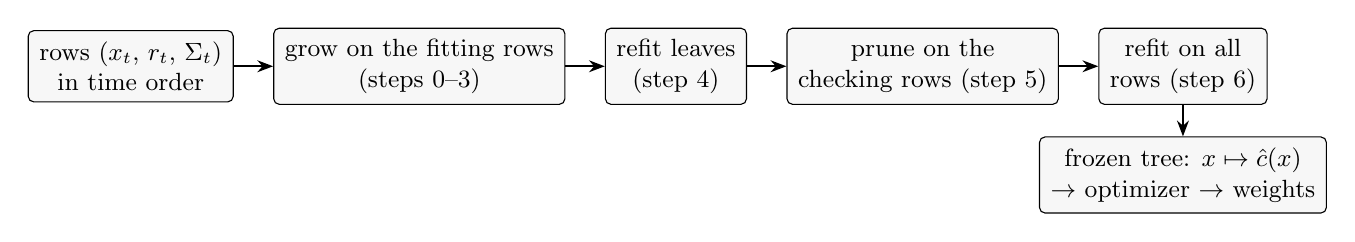
\begin{tikzpicture}[node distance=4mm and 5mm, every node/.style={font=\small},
  box/.style={draw, rounded corners=2pt, align=center, inner sep=4pt, fill=black!3},
  arr/.style={-{Stealth[length=2mm]}, thick}]
\node[box] (rows) {rows $(x_t,\,r_t,\,\Sigma_t)$\\in time order};
\node[box, right=of rows] (grow) {grow on the fitting rows\\(steps 0--3)};
\node[box, right=of grow] (refit) {refit leaves\\(step 4)};
\node[box, right=of refit] (prune) {prune on the\\checking rows (step 5)};
\node[box, right=of prune] (final) {refit on all\\rows (step 6)};
\node[box, below=of final] (use) {frozen tree: $x\mapsto\hat c(x)$\\$\to$ optimizer $\to$ weights};
\draw[arr] (rows) -- (grow); \draw[arr] (grow) -- (refit); \draw[arr] (refit) -- (prune); \draw[arr] (prune) -- (final); \draw[arr] (final) -- (use);
\end{tikzpicture}}
\end{figure}

\section{Inputs}\label{sec:inputs}
Training sees $T$ rows in time order, one per decision $t=1,\dots,T$:
\begin{itemize}\setlength{\itemsep}{1pt}
\item $x_t\in\R^p$: the features known on the decision day;
\item $r_t\in\R^n$: the simple returns of the $n$ assets from this decision to the next ($2\le n\le4$);
\item $\Sigma_t\in\R^{n\times n}$: a covariance of $r_t$ estimated from the past only, positive definite.
\end{itemize}
Real data (\code{weekly_rows}): decisions at the close of a fixed weekday, $r_t=P_{d_t+7}/P_{d_t}-1$, and $\Sigma_t=7\,\widehat{\mathrm{Cov}}(\text{last }H\text{ daily returns})+\varepsilon I$ with $H=180$, $\varepsilon=10^{-6}$; features are read on the decision day and must not use later data. The synthetic test (\code{recovery_test.py}) builds the same rows with a decision every $h$ days: $r_t=S_{t+h}/S_t-1$, $\Sigma_t=\mathrm{diag}(h\hat\sigma_t^2,\varepsilon)$ with the second asset cash. The last \code{test_periods} rows are held out; everything below sees the training rows only.

The decision problem has three parameters: the fee per traded notional $f\in\R^n_{\ge0}$ (one value per asset), the risk aversion $\lambda>0$ and the cap per asset $\bar w$. The holdings before the first decision are $u_1=\1/n$ unless given.

\textbf{Fitting and checking rows.} With \code{validation_fraction}${}=\rho_v>0$ the training rows are cut in time order: the first $T_f=T-\mathrm{round}(\rho_vT)$ are the \emph{fitting rows}, on which the tree is grown; the last $T-T_f$ are the \emph{checking rows}, which only prune it (step~5) and enter the final refit (step~6).

\section{Features: what the tree needs}\label{sec:features}
The code prescribes no feature; it reads the array $x_t$. What the training does with a feature decides what makes a good one.
\begin{itemize}\setlength{\itemsep}{1pt}
\item \textbf{Only the ordering matters.} A split is $x_j\le\theta$ with $\theta$ between two observed values (Section~\ref{sec:thresholds}); any increasing transformation (log, rank, scaling) gives the same partitions and the same leaf scores. No normalisation is needed, and a threshold on a price \emph{level} has no meaning out of sample: use stationary quantities (returns, ratios, volatilities, z-scores).
\item \textbf{The model is piecewise constant}: a tree of depth $D$ has at most $2^D$ leaves, hence $2^D$ score vectors. A feature should describe a \emph{state} of the market, not a fine forecast; two nested splits capture one interaction (``calm and rising'' against ``calm and falling''), which is the case a tree represents and a one-feature rule cannot.
\item \textbf{With fully invested weights only differences matter}: $w^\star(c+\alpha\1)=w^\star(c)$ (Section~\ref{sec:decision}). With two risky assets a feature is useful to the extent that it predicts the \emph{difference} of their returns; a cash column is what lets a feature reduce the exposure to the market.
\item \textbf{Every feature adds candidate splits, and the best of many looks good by luck.} With $N$ rows and a minimum leaf of $m$, each feature brings about $N-2m$ thresholds; five features give over a thousand candidates at the root of a 15-year weekly fit, and on data with no signal the best of them still lowers the in-sample regret. Hence few features, each with an economic reason, and the quantile or soft options of Section~\ref{sec:thresholds} when the candidates must be tamed. A pure-noise column fitted separately is a cheap diagnostic.
\item \textbf{Persistence sets the useful trading rate.} A feature that crosses its threshold often creates leaf changes, and each one can move the whole portfolio and pay the fee on both legs. The synthetic test (recovery note, Sections~4 and~8) gives the orders of magnitude: with a feature whose half-life is about a month, the threshold is recovered from daily to monthly decisions; with a half-life of a week, monthly decisions lose most of the value because the regime flips inside the holding period. Deciding more often than the feature moves adds fees, not information.
\item \textbf{What can be found at all.} With 15 years of daily data and a volatility of 1\% a day, a regime drift of $\pm25\%$ a year is recovered reliably, $\pm13\%$ a year about three times out of four and imprecisely, $\pm5\%$ a year not at all. A feature whose edge is below a few basis points a day will not be learnt by this or any other method from that much history; test it with the planted-threshold protocol before trading it.
\end{itemize}
Practical candidates, to be validated on real data: momentum of each asset and of their ratio over one to three months, realised-volatility regime, drawdown from the recent high, and volume or funding-rate indicators if the data are reliable.

\section{The decision problem}\label{sec:decision}
Given scores $c\in\R^n$, holdings $u$ and a covariance $\Sigma$, the portfolio is
\begin{equation}\label{eq:opt}
w^\star(c;u,\Sigma)=\argmax_{w\in\W}\;c^\top w-f^\top|w-u|-\lambda\,w^\top\Sigma w,
\qquad \W=\{w\in\R^n:\ 0\le w_i\le\bar w,\ \1^\top w=1\}.
\end{equation}
It is solved exactly: at the optimum each weight is at $0$, at $\bar w$, at $u_i$ (the fee puts a kink there) or free on one side of $u_i$; each of the $5^n$ patterns gives a small linear system, every admissible solution is feasible, and the best one is the unique optimum since the objective is strictly concave. All rows are solved in one vectorised call (\code{PortfolioOptimizer.solve}).

With two assets (asset $a$ and $b$, holding $v$ of $a$, $\Delta c=c_a-c_b$, $\phi=f_a+f_b$, $\kappa=2\lambda(\sigma_a^2+\sigma_b^2-2\sigma_{ab})$, minimum-variance weight $\bar a$ and $D=\Delta c-\kappa(v-\bar a)$):
\begin{equation}\label{eq:twoasset}
w_a=\begin{cases} v & |D|\le\phi\quad\text{(no trade)},\\[2pt] \bar a+\dfrac{\Delta c-\phi\,\mathrm{sign}(D)}{\kappa} & \text{otherwise,}\end{cases}\qquad\text{clipped to }[1-\bar w,\bar w].
\end{equation}
So a leaf acts through one number $\Delta c$, the position is linear in it with slope $1/\kappa$, and the no-trade band has half-width $\phi$. Only differences between scores matter: $w^\star(c+\alpha\1)=w^\star(c)$.

\section{The loss: decision regret}\label{sec:loss}
The utility of a decision $w$ in row $t$ and the regret of scores $c$ are
\begin{align}
U_t(w)&=r_t^\top w-f^\top|w-u_t|-\lambda\,w^\top\Sigma_t w,\label{eq:utility}\\
\Reg_t(c)&=U_t\big(w^\star(r_t;u_t,\Sigma_t)\big)-U_t\big(w^\star(c;u_t,\Sigma_t)\big)\ \ge0 .\label{eq:regret}
\end{align}
The first term is the best decision in hindsight from the same holdings $u_t$ (a one-period oracle). The holdings $u_t$ come from the replay of the current tree (Section~\ref{sec:path}) and are frozen while a round of the search runs. A row regret below $-10^{-6}$ aborts the fit (solver check); values in $[-10^{-6},0)$ are set to $0$.

\section{The path and the Sharpe ratio}\label{sec:path}
Scores $c_1,\dots,c_T$ are traded in time order from $u_1$:
\begin{equation}\label{eq:path}
w_t=w^\star(c_t;u_t,\Sigma_t),\qquad \pi_t=r_t^\top w_t-f^\top|w_t-u_t|,\qquad u_{t+1}=\frac{w_t\circ(1+r_t)}{1+r_t^\top w_t}.
\end{equation}
Holdings drift between decisions, so fees are paid on every difference $|w_t-u_t|$. The Sharpe ratio of a path is $S=\mathrm{mean}(\pi)/\mathrm{std}(\pi)$ per decision (divisor $T-1$, no risk-free rate); it is undefined with fewer than two rows, and it is $0$ for a path with constant zero net returns (all cash, no trade), so that a split can be judged against an all-cash tree. The replay also returns every row's regret~\eqref{eq:regret} along the path.

\section{The tree and its score}\label{sec:tree}
A tree of depth at most $D$ has internal nodes that split on one feature and leaves $\ell$ that hold one score vector $\hat c_\ell\in[-b,b]^n$ ($b={}$\code{prediction_bound}). The scores are not forecasts: they are the inputs that make the optimizer take the right decision on the rows of the leaf.

\textbf{Membership.} A split node $\nu$ on feature $j$ holds candidate thresholds $\theta_1<\dots<\theta_K$ with weights $\pi_1,\dots,\pi_K$ summing to 1 (one threshold with weight 1 for a plain split). A row with feature value $x$ goes left with weight
\begin{equation}\label{eq:membership}
\mu_\nu(x)=\sum_{k:\,\theta_k\ge x}\pi_k\in[0,1],
\end{equation}
that is, the weight of the thresholds at or above $x$, and right with weight $1-\mu_\nu(x)$. For a plain split $\mu_\nu(x)=\1\{x\le\theta\}$. The weight of row $t$ in leaf $\ell$ is the product of the memberships along the path from the root, $\omega_{t\ell}$; with plain splits every $\omega_{t\ell}\in\{0,1\}$ and each row is in exactly one leaf. The score of row $t$ is the mixture
\begin{equation}\label{eq:score}
\hat c(x_t)=\sum_\ell\omega_{t\ell}\,\hat c_\ell ,
\end{equation}
a piecewise-constant function of $x$ for a plain tree, a continuous and monotone one between two leaves for a soft one. $I_\ell=\{t:\omega_{t\ell}>0\}$ are the rows of leaf $\ell$ and $N_\ell=\sum_t\omega_{t\ell}$ its mass. A split node also reports one threshold, the $\pi$-weighted median of its candidates, and a \emph{spread}, the distance between its 25\% and 75\% weight quantiles ($0$ for a plain split).

\section{Fitting one leaf}\label{sec:leaf}
With the holdings frozen, the score of leaf $\ell$ minimises its weighted regret:
\begin{equation}\label{eq:leaf}
\hat c_\ell\approx\argmin_{c\in[-b,b]^n}L_\ell(c),\qquad L_\ell(c)=\sum_{t\in I_\ell}\omega_{t\ell}\,\Reg_t(c).
\end{equation}
The search is deterministic (\code{_fit_leaf}): start from the $\omega$-weighted mean of $r_t$ over $I_\ell$, clipped to $[-b,b]$; if a fallback vector is given, take it instead when it is strictly better (the fallback is the refitted parent for a child, the leaf's own vector for a refit, none for the root); then run 3 passes in which each coordinate in turn is moved to the best of 7 equally spaced values, the first pass over $[-b,b]$ and the next ones over a window of half-width $2b/6^k$ around the current best. One fit costs $2+3\cdot7n$ evaluations of $L_\ell$, each a vectorised solve over the leaf.

\section{Candidate thresholds}\label{sec:thresholds}
At a node with rows $I$ and weights $\omega$ (mass $N=\sum\omega$), the minimum mass of a child is $m_\ast=\max(m,\lceil\varphi N\rceil)$ with $m={}$\code{min_samples_leaf} and $\varphi={}$\code{min_leaf_fraction}. For feature $j$:
\begin{enumerate}\setlength{\itemsep}{1pt}
\item[(a)] \textbf{Plain.} The candidates are the midpoints between consecutive distinct values of $x_{tj}$, $t\in I$, whose two sides both carry a mass of at least $m_\ast$. With \code{max_thresholds}${}=M$ set, an evenly spaced subset by rank of size $M$ is kept.
\item[(b)] \textbf{Quantiles} (\code{threshold_quantiles}${}=(q_1,\dots,q_Q)$). Only the candidates of (a) nearest to the quantiles $q_1,\dots,q_Q$ of the node's values are kept.
\item[(c)] \textbf{Refinement} (\code{refine_thresholds}). After the screen of (b), let $\theta_\circ$ be the best quantile candidate; every candidate of (a) strictly between the two quantile candidates neighbouring $\theta_\circ$ is screened as well. With plain splits the best of them, $\theta_\bullet$, replaces $\theta_\circ$ only if $Q(\theta_\circ)-Q(\theta_\bullet)>k\,\mathrm{se}\big(Q(\theta_\bullet)-Q(\theta_\circ)\big)$ with $k={}$\code{refine_standard_errors}; with soft splits they simply join the candidate set.
\end{enumerate}
\textbf{The screen.} Each candidate $\theta$ is scored cheaply: each child gets its clipped $\omega$-weighted mean return as scores, and
\begin{equation}\label{eq:screen}
Q(\theta)=\sum_{t\in I}\omega_t\,\Reg_t\big(c_{\mathrm{side}(t)}(\theta)\big),\qquad
c_{\mathrm{left}}(\theta)=\mathrm{clip}\Big(\tfrac{\sum_{x_{tj}\le\theta}\omega_tr_t}{\sum_{x_{tj}\le\theta}\omega_t},\pm b\Big),
\end{equation}
and likewise on the right. The standard error of a difference of two such sums is $\mathrm{se}=\sqrt{|I|}\,\mathrm{std}_t\big(\delta_t\big)$ with $\delta_t$ the per-row difference of the two regrets (rows treated as independent).

\textbf{Plain splits} (\code{smoothing}${}=0$): the \code{shortlist_size} candidates with the smallest $Q$ over all features go to the full fit of step~1c; each has one threshold with weight $1$.

\textbf{Soft splits} (\code{smoothing}${}=\kappa>0$). For each feature, all its candidates $\theta_1<\dots<\theta_K$ are kept together with Boltzmann weights
\begin{equation}\label{eq:boltzmann}
z_k=\frac{Q(\theta_k)-\min_lQ(\theta_l)}{\mathrm{se}\big(Q(\theta_k)-\min_lQ(\theta_l)\big)},\qquad
\pi_k=\frac{e^{-z_k/\kappa}}{\sum_le^{-z_l/\kappa}},
\end{equation}
so that thresholds the data cannot tell apart from the best one (small $z$) share the weight and clearly worse ones get none ($z_k=0$ when the regrets are identical, $\infty$ when they differ with zero standard error). The feature yields one candidate split, ranked by its best $Q$; its children receive the rows with $\mu>0$ on the left with weights $\omega\mu$ and the rows with $\mu<1$ on the right with weights $\omega(1-\mu)$, by~\eqref{eq:membership}. As $\kappa\to0$ the weight concentrates on the best candidate and the split is the plain one.

\section{Training, step by step}\label{sec:steps}
\textbf{Algorithm} (\code{fit}). Steps 0 to 4 see the fitting rows only.
\begin{enumerate}\setlength{\itemsep}{2pt}
\item[0.] \textbf{Root.} Fit one score vector on all fitting rows with~\eqref{eq:leaf}, the holdings being $u_t=\1/n$ for every row. Replay the tree~\eqref{eq:path}: this gives the holdings $u_t$ the tree would really have had, the hindsight utilities of~\eqref{eq:regret} and the Sharpe ratio $S$. Regrets are measured from these holdings until the next acceptance.
\item[1.] \textbf{For every leaf} $\ell$ of depth $<D$ and mass $N_\ell\ge2m_\ast$:
  \begin{enumerate}\setlength{\itemsep}{1pt}
  \item[a.] \emph{Parent refit.} Refit $\ell$ on the current holdings: $\hat c_\ell^{\,\mathrm{refit}}$ (a yardstick and the children's fallback; never written into the tree).
  \item[b.] \emph{Candidates.} Build the candidate thresholds of every feature (Section~\ref{sec:thresholds}), screen them with~\eqref{eq:screen}, and shortlist: the best \code{shortlist_size} thresholds (plain) or one weighted set per feature (soft).
  \item[c.] \emph{Children.} For each shortlisted split, route the rows with~\eqref{eq:membership}, fit both children with~\eqref{eq:leaf}, and compute the regret reduction
  $\Delta=L_\ell(\hat c_\ell^{\,\mathrm{refit}})-L_{\mathrm{left}}(\hat c_{\mathrm{left}})-L_{\mathrm{right}}(\hat c_{\mathrm{right}})$.
  Keep the split if $\Delta/N_\ell>\varepsilon_R$ (\code{min_regret_improvement}).
  \end{enumerate}
\item[2.] \textbf{Choice and confirmation.} Sort the kept splits of all leaves by $\Delta$, largest first (SPOT's criterion). For the first one, rebuild the scores~\eqref{eq:score} of the tree with that split and replay it; accept it if $S'>S+\varepsilon_S$ (\code{min_sharpe_improvement}); otherwise try the next. If none passes, growth stops.
\item[3.] After an acceptance the replay of the new tree gives the new $u_t$, hindsight utilities and $S$; return to step~1. The rows and weights of the two children are those of step~1c.
\item[4.] \textbf{Refit on the final holdings.} Refit every leaf with~\eqref{eq:leaf} (fallback: its own vector); keep the new vectors only if the replayed Sharpe ratio does not fall.
\item[5.] \textbf{Pruning on the checking rows} ($\rho_v>0$), from the bottom of the tree up. For a split node $\nu$: let $\mathcal T$ be the current tree (the split at $\nu$ with every surviving split below it) and $\mathcal T_{\nu\to\mathrm{leaf}}$ the same tree with $\nu$ as a single leaf, its vector fitted with~\eqref{eq:leaf} on the fitting rows of $\nu$ (weights $\omega$), from the holdings of $\mathcal T$ replayed on the fitting rows. Each tree trades the fitting rows, then the checking rows from the holdings it ends with. On the checking rows only,
\begin{equation}\label{eq:prune}
\text{the split stays}\iff \overline{\Reg}^{\,\mathrm{chk}}(\mathcal T_{\nu\to\mathrm{leaf}})-\overline{\Reg}^{\,\mathrm{chk}}(\mathcal T)>\varepsilon_R\ \text{ and }\ S^{\mathrm{chk}}(\mathcal T)>S^{\mathrm{chk}}(\mathcal T_{\nu\to\mathrm{leaf}})+\varepsilon_S ,
\end{equation}
otherwise $\nu$ becomes that leaf. A split is judged with everything below it; a split no checking row reaches cannot be confirmed.
\item[6.] \textbf{Refit on all training rows.} The rules are settled: all $T$ rows are routed through the pruned tree with~\eqref{eq:membership}, the tree is replayed, every leaf vector is refitted with~\eqref{eq:leaf} on its rows (fitting and checking, fallback its own vector). This refit is always kept, since the vectors it replaces never saw the checking rows. Leaf masses $N_\ell$ then count all training rows.
\end{enumerate}

Two remarks. Within a round, regrets are measured on the holdings of the tree \emph{without} the candidate split; the change of path a split causes is seen by the Sharpe replay of step~2 and by the next round. And there is no single objective: leaf vectors minimise regret, the structure follows the largest regret reduction, the Sharpe ratio confirms on the fitting rows, the checking rows prune. Both tests of step~2 are in-sample; the pruning of step~5 is the out-of-sample judge. The logs \code{growth_log} and \code{pruning_log} record every accepted split and every pruning decision.

\section{Using the tree}\label{sec:use}
A frozen tree maps features to scores by~\eqref{eq:score} (\code{predict_returns}); the weights are $w^\star(\hat c(x);u,\Sigma)$ with the current holdings and covariance (\code{predict_weights}). A backtest is the replay~\eqref{eq:path} of those scores (\code{replay}); \code{train_and_test} fits on all rows but the last \code{test_periods}, replays the training rows from $u_1=\1/n$, then the test rows from the holdings the training replay ends with, against the same tree without splits and an equal-weight portfolio rebalanced every period.

\section{Parameters}\label{sec:parameters}
\begin{table}[H]
\centering\small
\begin{tabularx}{\linewidth}{@{}>{\raggedright\arraybackslash}p{4.9cm} c c c L@{}}
\toprule
Parameter & default & \code{run.py} & note & role\\
\midrule
\code{max_weight} $\bar w$ & 1 & 1 & 1 & cap per asset; long-only, fully invested\\
\code{fee_rate} $f$ & 0.001 & 0.0003 & (0.0003, 0) & fee per traded notional, scalar or per asset\\
\code{risk_aversion} $\lambda$ & 1 & 1 & 1 & multiplies $w^\top\Sigma w$; positions are interior in a score window of width $2\lambda\sigma_h^2$\\
\code{max_depth} $D$ & 4 & 2 & 2 & root is depth 0\\
\code{min_samples_leaf} $m$ & 10 & 20 & 20 & minimum rows (mass) per leaf\\
\code{min_leaf_fraction} $\varphi$ & 0 & 0 & 0 & minimum share of the node's mass per child\\
\code{max_thresholds} $M$ & 10 & \code{None} & \code{None} & candidates per feature; \code{None} screens all\\
\code{threshold_quantiles} & \code{None} & \code{None} & \code{None} & quantile candidates only, e.g.\ deciles\\
\code{refine_thresholds} & off & off & off & local refinement around the best quantile\\
\code{refine_standard_errors} $k$ & 0 & 0 & 0 & hurdle of the refinement for plain splits\\
\code{smoothing} $\kappa$ & 0 & 0 & 0 & soft splits with Boltzmann weights~\eqref{eq:boltzmann}; 0 = plain\\
\code{shortlist_size} & 3 & 3 & 3 & screened splits per leaf that get a full fit (plain splits)\\
\code{min_regret_improvement} $\varepsilon_R$ & $10^{-6}$ & $10^{-6}$ & $10^{-6}$ & gate on $\Delta/N_\ell$ in growth, on the mean checking regret in pruning\\
\code{min_sharpe_improvement} $\varepsilon_S$ & 0 & 0 & 0 & margin on the Sharpe ratio, in growth and in pruning\\
\code{validation_fraction} $\rho_v$ & 0 & 0.25 & 0.25 & last share of the training rows that prunes; 0 = no pruning\\
\code{prediction_bound} $b$ & 0.10 & 0.10 & 0.10 & leaf vectors in $[-b,b]^n$\\
\code{search_passes}, \code{search_grid_size} & 3, 7 & 3, 7 & 3, 7 & leaf search\\
\code{regret_tolerance} & $10^{-6}$ & $10^{-6}$ & $10^{-6}$ & numerical guard on row regrets\\
\bottomrule
\end{tabularx}
\caption{The parameters: class defaults, the values of \code{run.py} (real data), and those of the recovery note (\code{recovery_test.py}, base case). Section~8 of the note varies $\lambda$, $f$, $D$ and the quantiles; its Section~9 the split-search options.}
\end{table}

\section{What changed since the pipeline report}\label{sec:changes}
\begin{itemize}\setlength{\itemsep}{1pt}
\item \textbf{Sharpe ratio of an all-cash path.} It was NaN, so every comparison ``with split $>$ without'' failed whenever the tree without the split sat in cash, and pruning removed such splits whatever their merit. It is now $0$ (Section~\ref{sec:path}).
\item \textbf{Leaves carry weights.} Internally a leaf is (node, rows, weights, depth); with plain splits all weights are 1 and nothing changes. Candidate scores in steps~2 and~4 are rebuilt from the leaves rather than updated in place, which keeps the plain case exact.
\item \textbf{Four options in the split search}, all off by default: quantile candidates with a minimum leaf fraction, local refinement with a standard-error hurdle, and soft splits with Boltzmann weights (Section~\ref{sec:thresholds}). A soft node stores its candidates, their weights and a spread; its reported threshold is the weighted median.
\item Everything else in the earlier description (decision problem, regret, path, leaf search, growth, pruning, final refit) is unchanged and is restated above.
\end{itemize}
\end{document}
